%!TEX program = xelatex

\documentclass[UTF8]{ctexart}
\usepackage{ctex}

\CTEXsetup[format={\Large\bfseries}]{section}

\usepackage[version=3]{mhchem} % Package for chemical equation typesetting
\usepackage{siunitx} % Provides the \SI{}{} and \si{} command for typesetting SI units
\usepackage{graphicx} % Required for the inclusion of images
\graphicspath{{assets/}}
\usepackage{natbib} % Required to change bibliography style to APA
\usepackage{amsmath} % Required for some math elements 
\usepackage{amssymb}
\usepackage[hidelinks]{hyperref}
\usepackage{makecell} % 3 Packages for flexible tabular
\usepackage{multirow}
\usepackage{multicol}

\usepackage{pdfpages}  % include pdf pages for original data etc.

\usepackage{geometry}% 版面大小
\geometry{a4paper,scale=0.7}

\usepackage{fontspec}

\setCJKfamilyfont{hwxk}{STXingkai}% 字体
\newcommand{\hwxk}{\CJKfamily{hwxk}}

\usepackage{fancyhdr}% 页眉页脚
\fancypagestyle{EE_Digital1Exp_template}{
    \fancyhead[L]{\Large {\hwxk 南京大学电子科学与工程学院}}
    \fancyhead[R]{数字系统1实验报告}
    \fancyfoot[c]{- \thepage \ -}
    \renewcommand\footrulewidth{0pt}
}

% 4级目录
\setcounter{secnumdepth}{4}
\setcounter{tocdepth}{4}

\usepackage{graphicx} % Packages for figures
\usepackage{caption2}
\usepackage{subfigure}
\usepackage{float}

\usepackage{listings} % Packages for code block
\usepackage{xcolor}

% for verilog code coloring
\definecolor{vgreen}{RGB}{104,180,104}
\definecolor{vblue}{RGB}{49,49,255}
\definecolor{vorange}{RGB}{255,143,102}

\lstdefinestyle{verilog-style}
{
    language=Verilog,
    basicstyle=\small\ttfamily,
    keywordstyle=\color{vblue},
    identifierstyle=\color{black},
    commentstyle=\color{vgreen},
    numbers=left,
    numberstyle=\tiny\color{black},
    numbersep=10pt,
    tabsize=8,
    moredelim=*[s][\colorIndex]{[}{]},
    literate=*{:}{:}1
}

\makeatletter
\newcommand*\@lbracket{[}
\newcommand*\@rbracket{]}
\newcommand*\@colon{:}
\newcommand*\colorIndex{%
    \edef\@temp{\the\lst@token}%
    \ifx\@temp\@lbracket \color{black}%
    \else\ifx\@temp\@rbracket \color{black}%
    \else\ifx\@temp\@colon \color{black}%
    \else \color{vorange}%
    \fi\fi\fi
}
\makeatother

\usepackage{trace}




%设置图片、表格编号
\renewcommand{\thetable}{\thesubsection{}-\arabic{table}}
\renewcommand{\thefigure}{\thesubsection{}-\arabic{figure}}
\renewcommand{\thefigure}{\thesubsection{}-\arabic{equation}}
\usepackage{amsmath}
\numberwithin{figure}{subsection}
\numberwithin{table}{subsection}
\numberwithin{equation}{subsection}

\setlength\parindent{6pt} % Removes all indentation from paragraphs

\renewcommand{\labelenumi}{\alph{enumi}.} % Make numbering in the enumerate environment by letter rather than number (e.g. section 6)

%\usepackage{times} % Uncomment to use the Times New Roman font

%----------------------------------------------------------------------------------------
%	DOCUMENT INFORMATION
%----------------------------------------------------------------------------------------

\title{\textbf{实验四\ 计数器:硬件电路}} % Title

\author{电子科学与工程学院\ 刘时宜\ 201180078} % Author name

\date{} % Date for the report

\begin{document}

\pagestyle{EE_Digital1Exp_template}

\maketitle % Insert the title, author and date

\begin{center}
    \begin{tabular}{l r}
    实验日期: & 2021年12月07日 \\ % Date the experiment was performed
    指导老师: & 高健 % Instructor/supervisor
    \end{tabular}
    \par 点击目录、书签栏、以及行文中的图表标号的均可跳转至相应页面
    \end{center}
    
% If you wish to include an abstract, uncomment the lines below
% \begin{abstract}
% Abstract text
% \end{abstract}

\tableofcontents

\section{实验目的}
\begin{enumerate}
    \item 利用计数器芯片与数码管搭建计数器硬件电路
\end{enumerate}

\section{实验仪器与主要器材}
\begin{center}
    \begin{tabular}{ll}
        \textbf{仪器:} & \\
        Basys3 FPGA 开发板 & 1台\\
        KEYSIGHT DSOX1102AG 示波器 & 1台\\
        示波器高频探头 & 1套\\
        ROGOL DM3068 万用表 & 1台\\
        \textbf{软件:} & \\
        Multisim & 14.1 \\
        \textbf{芯片:} & \\
        74LS90 & 1片 \\
        74LS47 & 1片 \\
        \textbf{耗材:} & \\
        导线 & 若干 \\
    \end{tabular}
\end{center}

\section{实验原理}
\par 计数器在数字系统中广泛使用,可以用于对时钟脉冲计数、分频、定时、进行数学运算等。
\par 计数器种类繁多。如果按照计数器中的触发器是否同时翻转分类,可以将计数器分为同步式和异步式两种。同步计数器中,当时钟脉冲输入时触发器的翻转同时发生,而在异步计数器中,触发器的翻转又先后,不是同时发生的。
\par 如果按照计数过程中数字的增减分类,可以分为加法计数器、减法计数器以及可逆计数器。随着计数脉冲的不断输入而作递增的计数器称为加法计数器,作递减计数的称为减法计数器,可增可减的称为可逆计数器。
\par 本实验中用到的计数器为异步加法计数器。将其接到BCD译码器及数码管,即可获得计数显示。

\section{实验过程}
\subsection{十进制计数器}
\subsubsection{原理电路}
\par 实验电路原理图如\ref{10 theory cir}所示。其中将74LS90的QA端接回INB触发端口,利用74LS90芯片特性构成十进制计数器。74LS90产生加法计数的BCD码后将其送至74LS47BCD显示译码器,进行译码并将输出送至数码管进行显示输出。

\begin{figure}[H]
    \begin{center}
        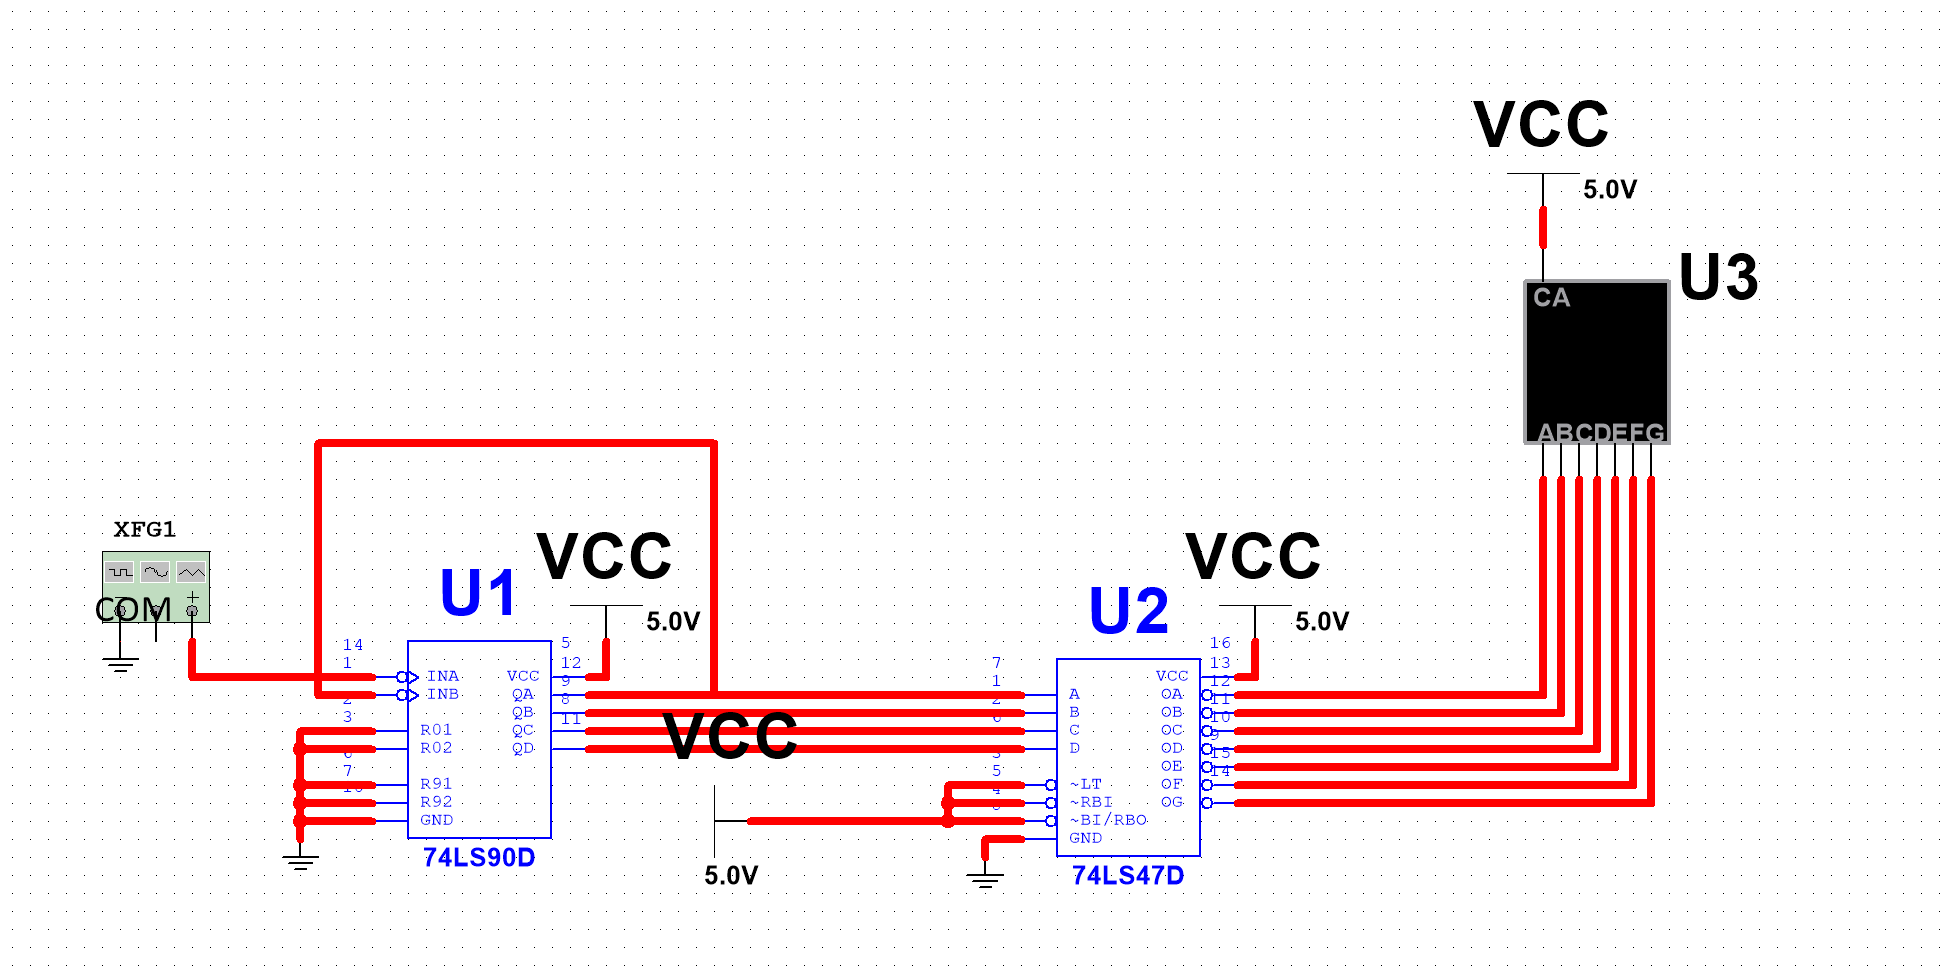
\includegraphics[width=0.8\textwidth]{design/10 circuit.png}
    \end{center}
    \caption{十进制计数器:原理电路}
    \label{10 theory cir}
\end{figure}

\subsubsection{电路实验}
\par 依据原理图,搭建硬件电路如图\ref{10 cir}所示。输入信号INA接信号发生器方波。方波参数为高电平\SI{5}{\volt},低电平\SI{0}{\volt},频率\SI{3}{\hertz}。

\begin{figure}[H]
    \begin{center}
        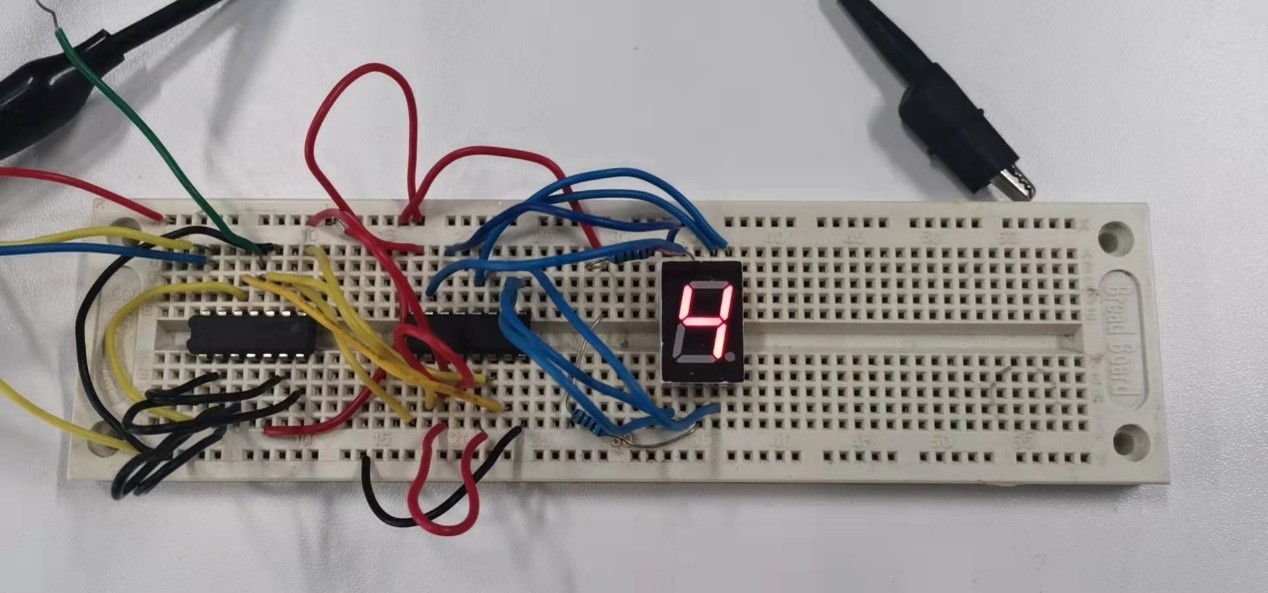
\includegraphics[width=0.8\textwidth]{10/circuit.jpg}
    \end{center}
    \caption{十进制计数器:硬件电路}
    \label{10 cir}
\end{figure}

\par 打开电源、打开信号源,观察实验现象。\SI{3}{\hertz}时电路现象已录制为"十进制计数器.mp4",附在邮件插件中。
\par 加大信号源频率,使用示波器观察计数器各引脚输出。其中信道1为时钟信号,信道2分别为各位输出。

\begin{figure}[H]
    \centering
    \subfigure[QA]{
    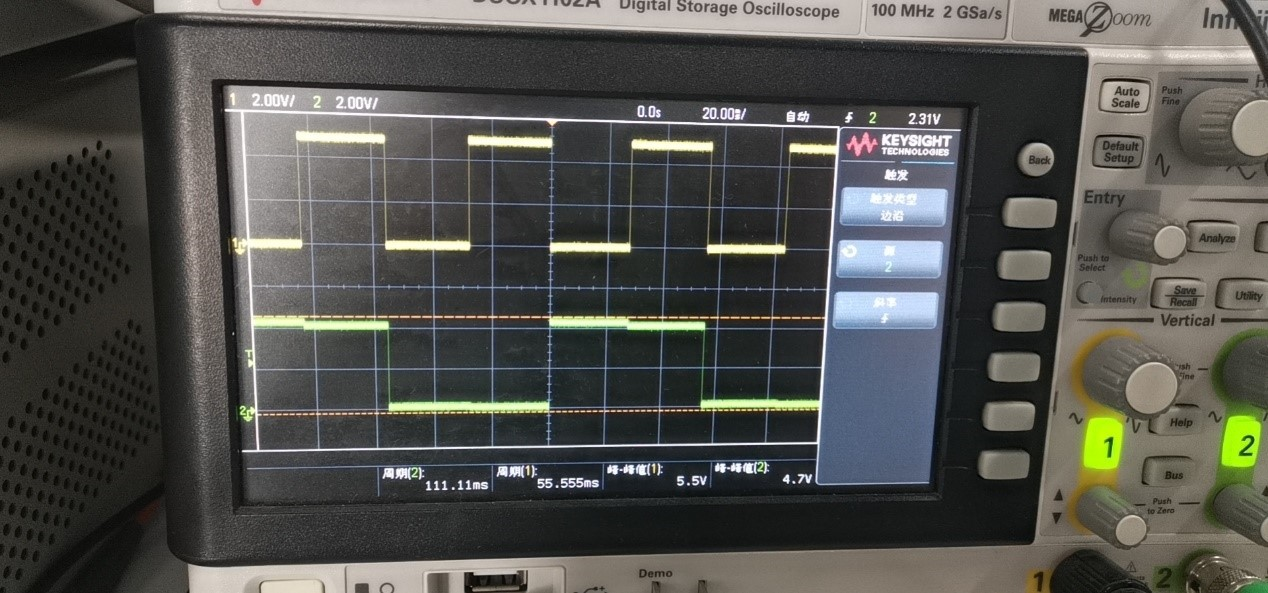
\includegraphics[width=0.45\textwidth]{10/QA.jpg}}
    \subfigure[QB]{
    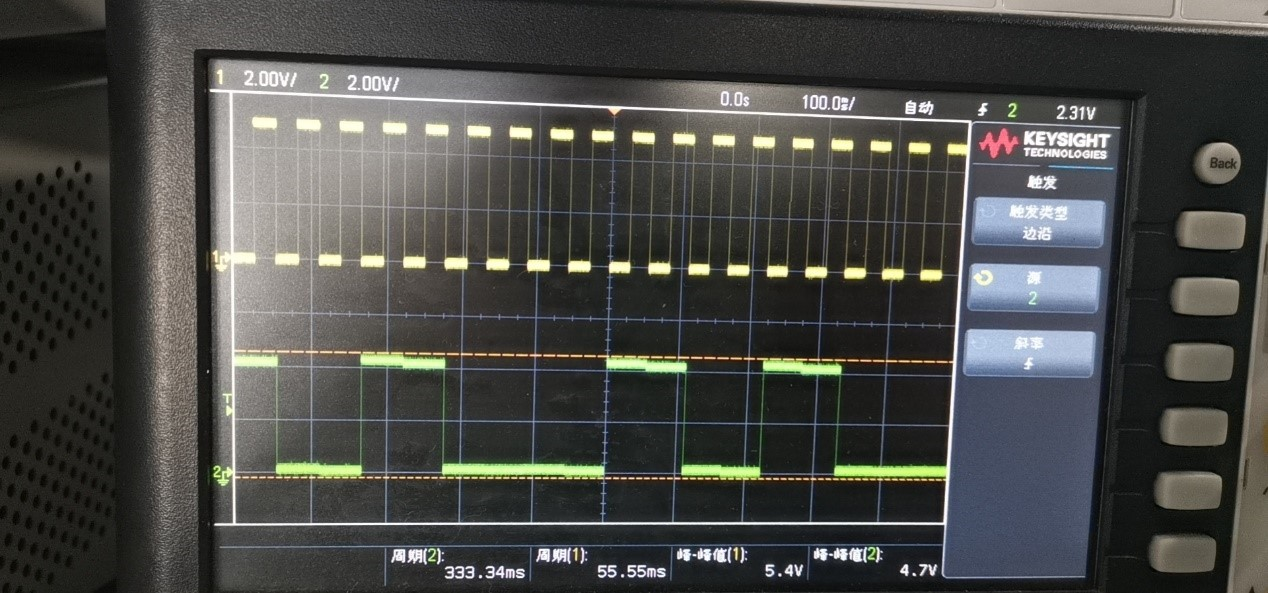
\includegraphics[width=0.45\textwidth]{10/QB.jpg}}
    \subfigure[QC]{
    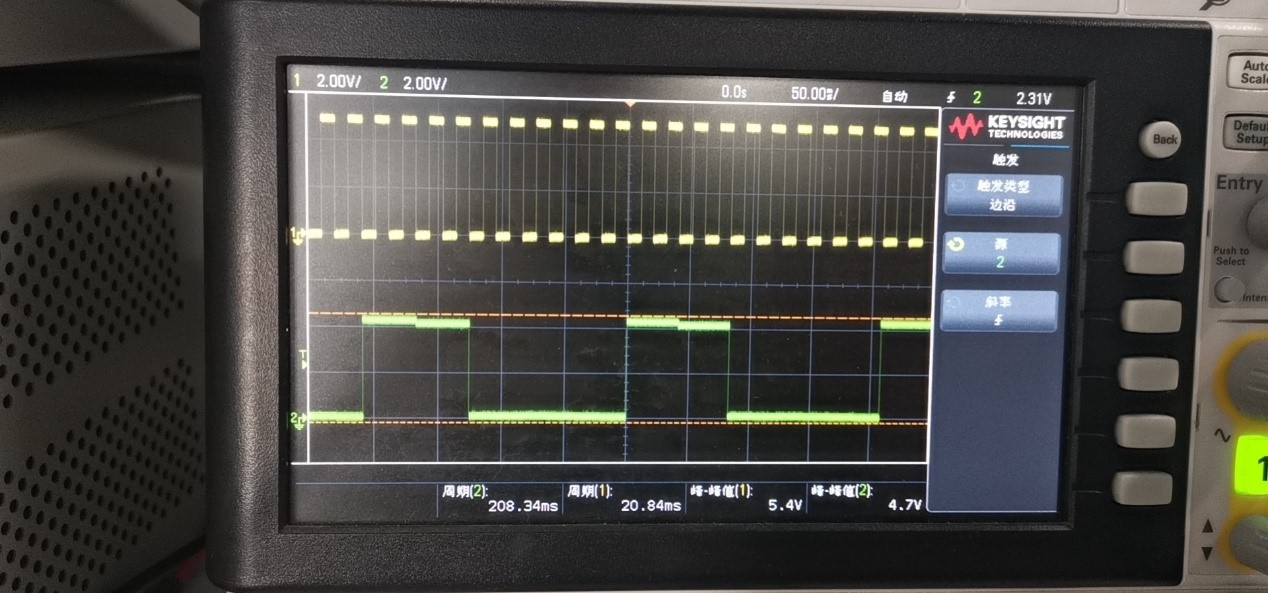
\includegraphics[width=0.45\textwidth]{10/QC.jpg}}
    \subfigure[QD]{
    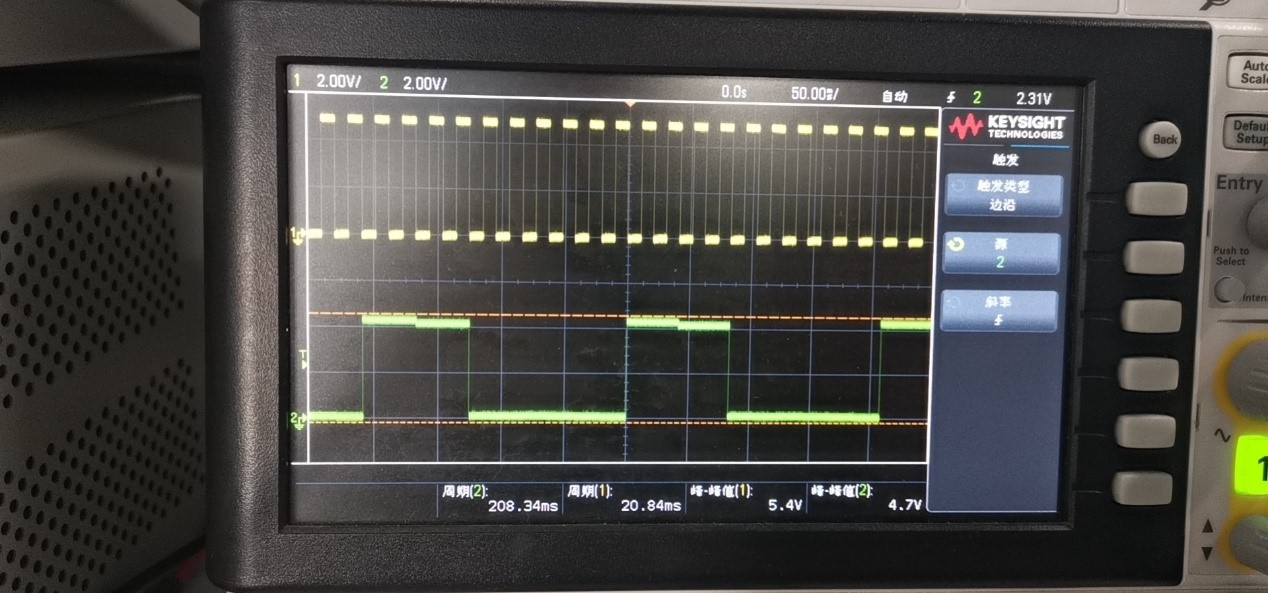
\includegraphics[width=0.45\textwidth]{10/QD.jpg}}
    \caption{十进制计数器:引脚波形}
    \label{10 osci}
\end{figure}

\par 可以看到,电路现象与各引脚波形与理论相符,成功搭建了十进制计数器硬件电路。


\subsection{十进制计数器}
\subsubsection{原理电路}
\par 实验电路原理图如\ref{10 theory cir}所示。其中将74LS90的QA端接回INB触发端口,利用74LS90芯片特性构成十进制计数器。74LS90产生加法计数的BCD码后将其送至74LS47BCD显示译码器,进行译码并将输出送至数码管进行显示输出。

\begin{figure}[H]
    \begin{center}
        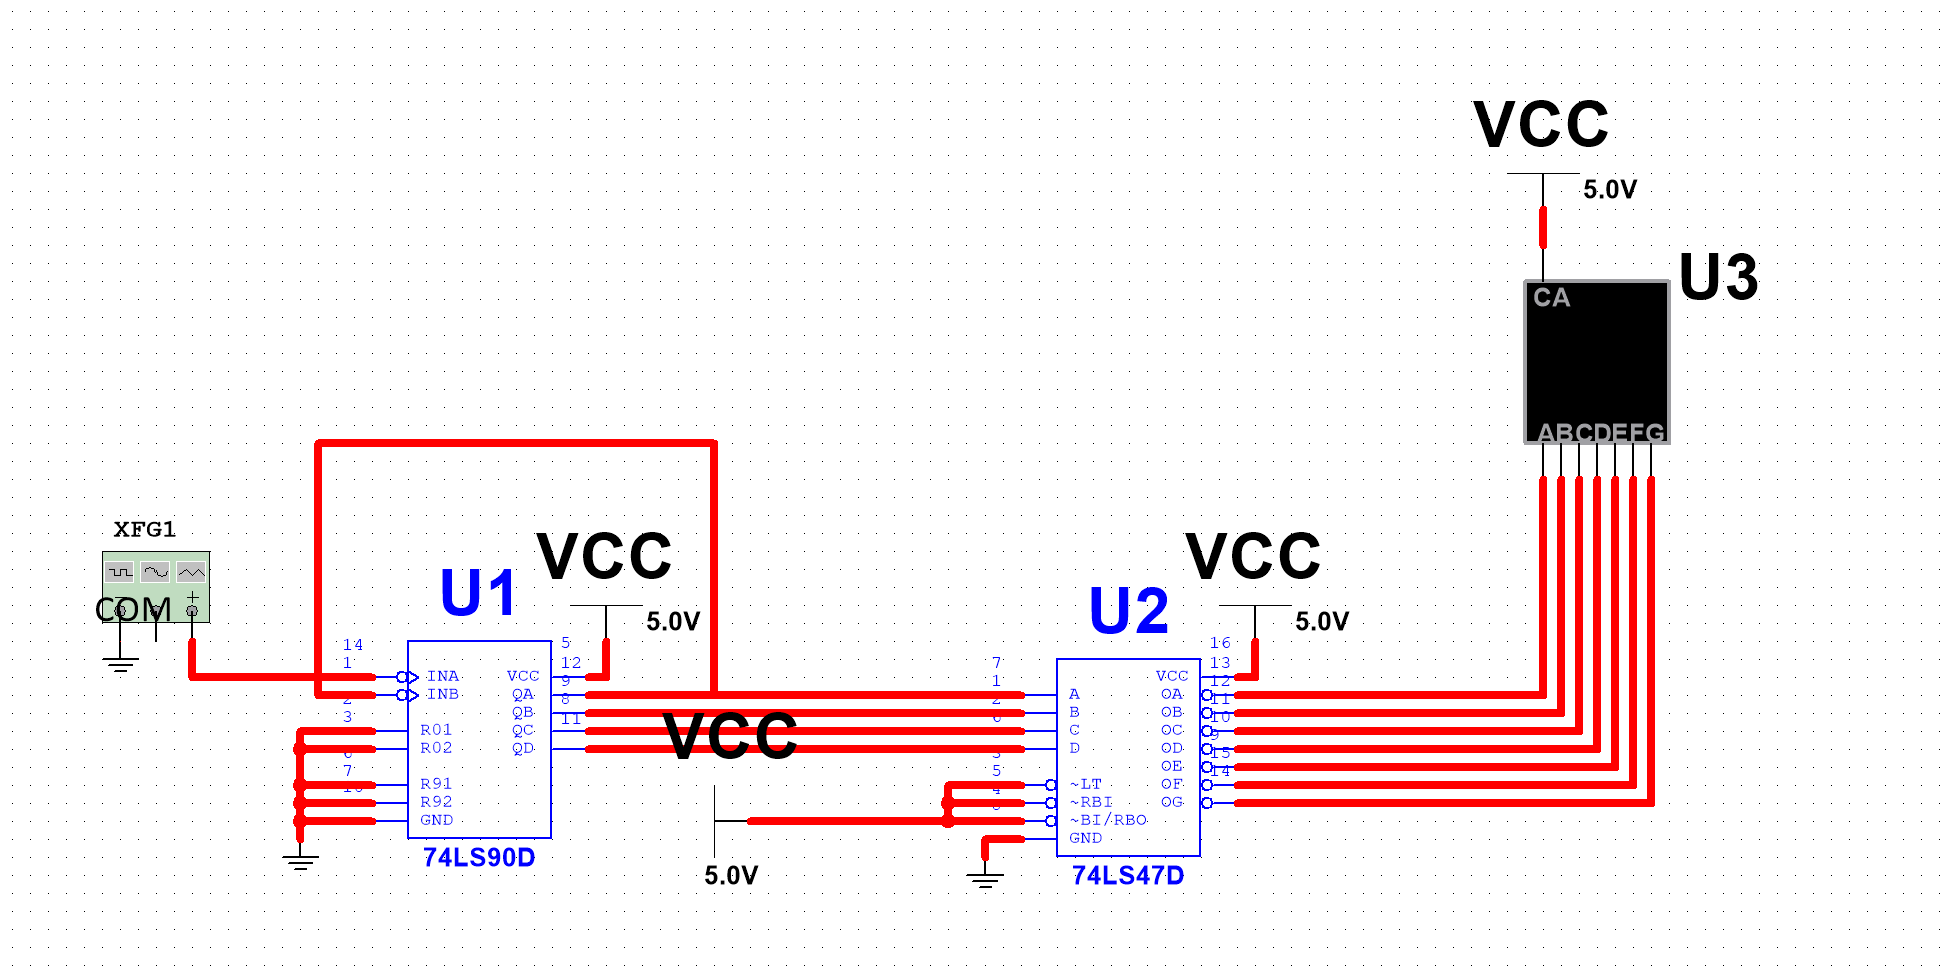
\includegraphics[width=0.8\textwidth]{design/10 circuit.png}
    \end{center}
    \caption{十进制计数器:原理电路}
    \label{10 theory cir}
\end{figure}

\subsubsection{电路实验}
\par 依据原理图,搭建硬件电路如图\ref{10 cir}所示。输入信号INA接信号发生器方波。方波参数为高电平\SI{5}{\volt},低电平\SI{0}{\volt},频率\SI{3}{\hertz}。

\begin{figure}[H]
    \begin{center}
        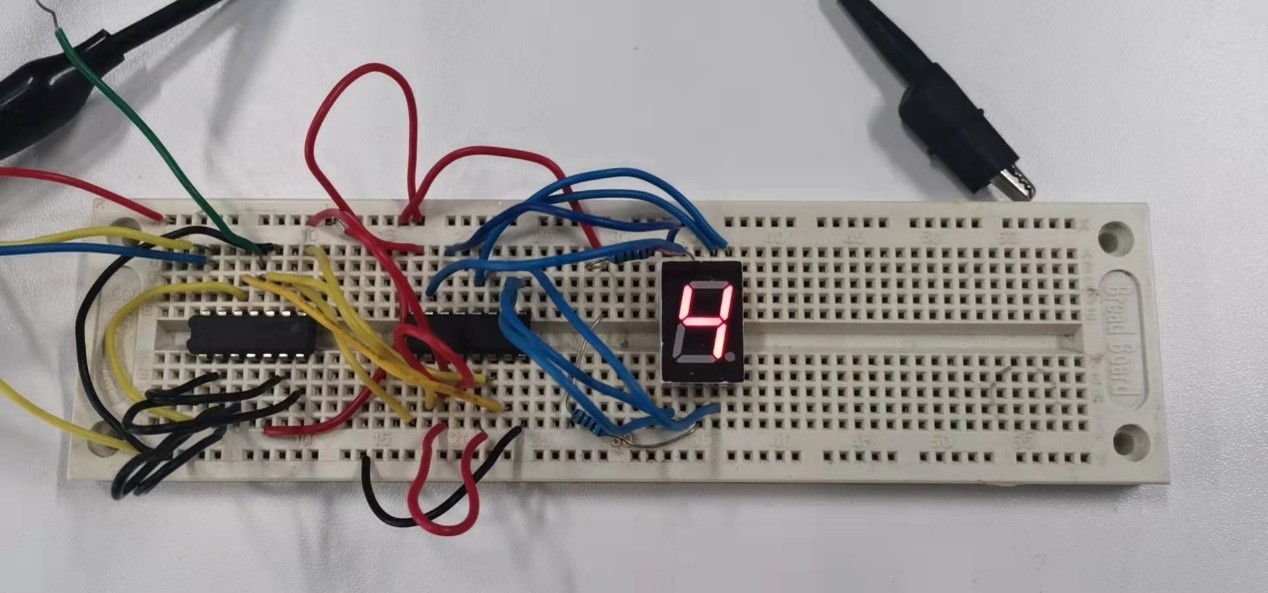
\includegraphics[width=0.8\textwidth]{10/circuit.jpg}
    \end{center}
    \caption{十进制计数器:硬件电路}
    \label{10 cir}
\end{figure}

\par 打开电源、打开信号源,观察实验现象。\SI{3}{\hertz}时电路现象已录制为"十进制计数器.mp4",附在邮件插件中。
\par 加大信号源频率,使用示波器观察计数器各引脚输出。其中信道1为时钟信号,信道2分别为各位输出。

\begin{figure}[H]
    \centering
    \subfigure[QA]{
    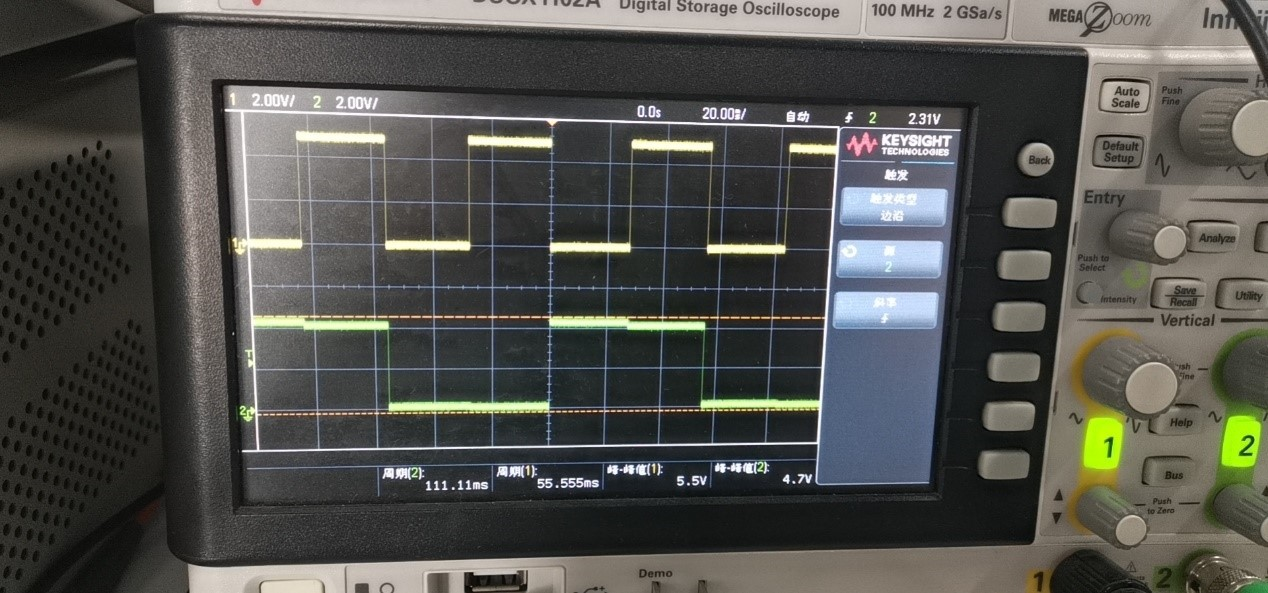
\includegraphics[width=0.45\textwidth]{10/QA.jpg}}
    \subfigure[QB]{
    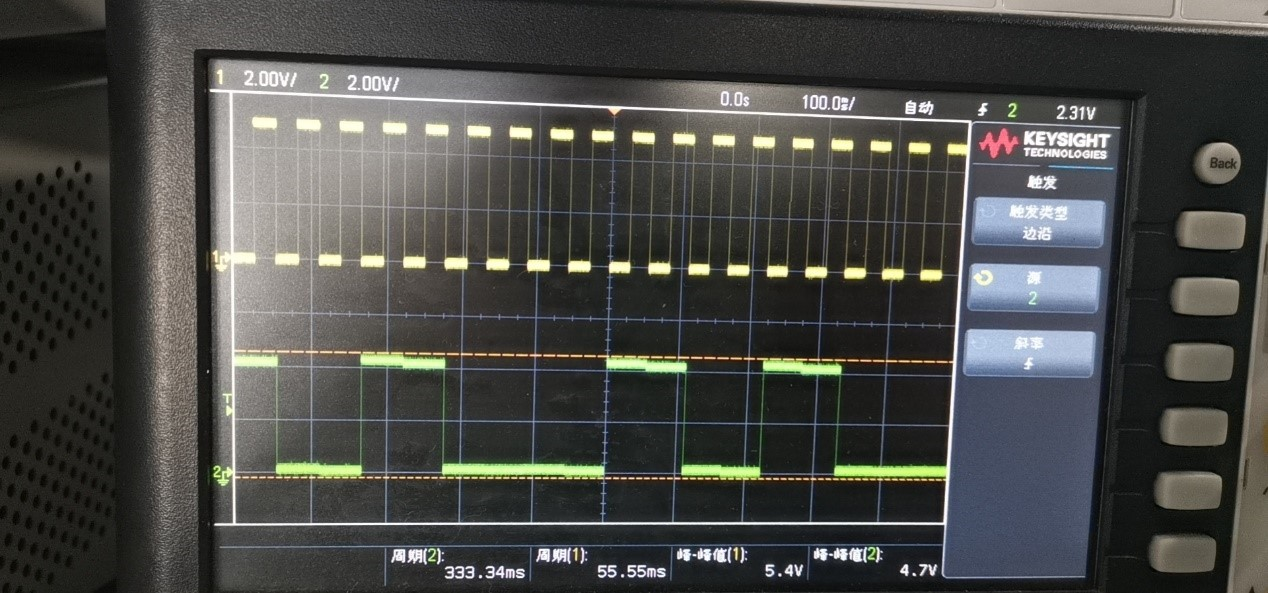
\includegraphics[width=0.45\textwidth]{10/QB.jpg}}
    \subfigure[QC]{
    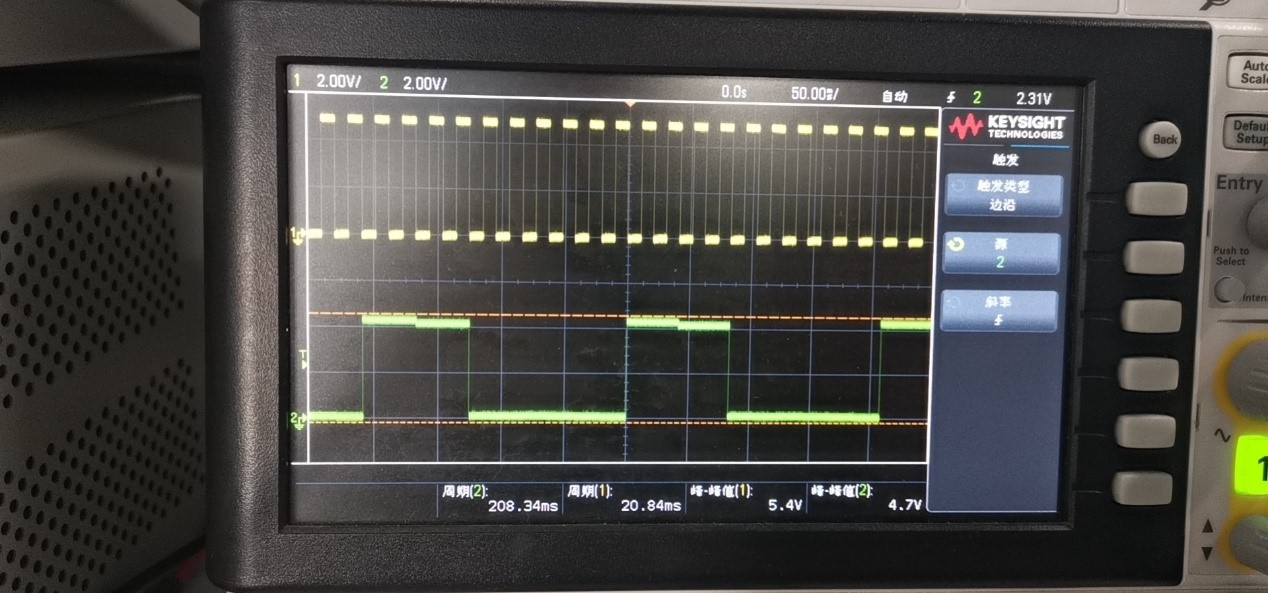
\includegraphics[width=0.45\textwidth]{10/QC.jpg}}
    \subfigure[QD]{
    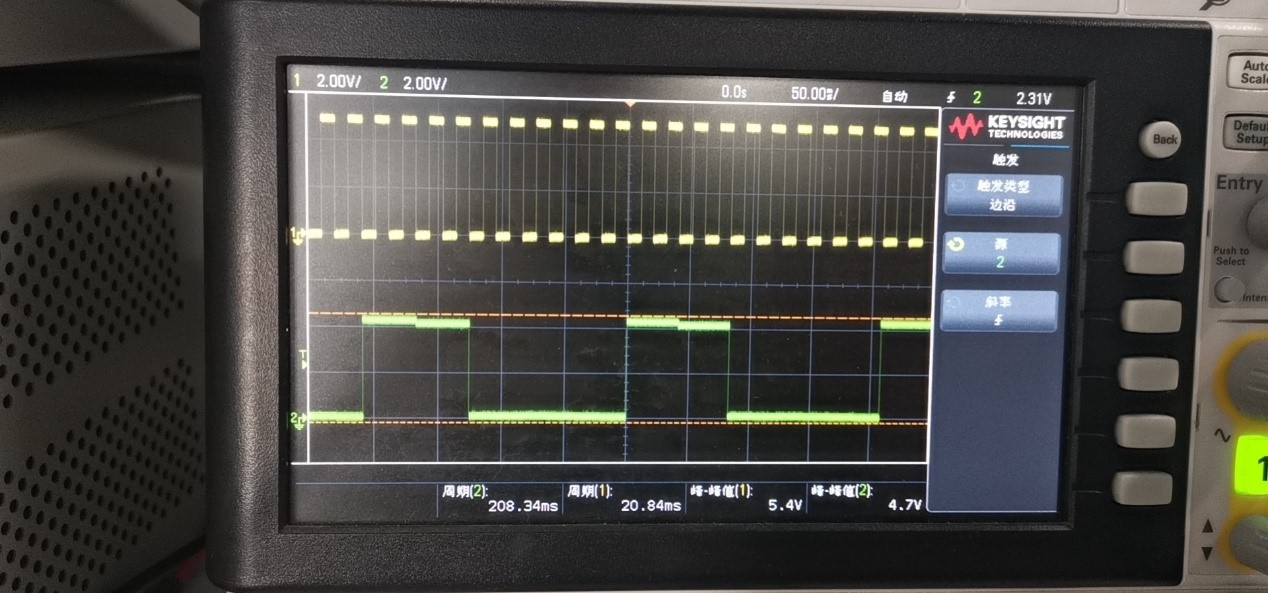
\includegraphics[width=0.45\textwidth]{10/QD.jpg}}
    \caption{十进制计数器:引脚波形}
    \label{10 osci}
\end{figure}

\par 可以看到,电路现象与各引脚波形与理论相符,成功搭建了十进制计数器硬件电路。



\section{实验总结}


\section*{原始数据}


\end{document}